\documentclass[12pt]{report}

\usepackage[french]{babel}

\usepackage[a4paper,top=2cm,bottom=2cm,left=2cm,right=2cm]{geometry}

\usepackage[T1]{fontenc}
\usepackage{amsmath}
\usepackage{graphicx}
\usepackage[colorlinks=true, allcolors=black]{hyperref}
\usepackage{titlesec}
\usepackage{lipsum}
\usepackage{ragged2e}
\usepackage{float}

\titleformat{\chapter}[display]{\raggedright\normalfont\bfseries}{}{0pt}{\huge}
% \titleformat{\section}[display]{\raggedright\normalfont\bfseries}{}{0pt}{\large}


\title{{\Huge Rapport de Projet} \\ \vspace{0.2cm} Modélisation et asservissement \\ du turboréacteur DGEN 380 }
\author{RICHELET Arthur
\\RENAYUD Maxime
\\FONTANELLE Dorian
\and
  DELMOTTE-DIAS Hélène
\\PASQUET Xavier}


% titre
\date{Encadrant: M. FARGUES \\ \vspace{0.5cm}
Décembre 2022 \\
\vspace{2cm}

\includegraphics[scale=0.4]{fig/evering_logo.jpg}}

\begin{document}

\maketitle

\tableofcontents


\newpage

\chapter{Abstract}

Le but de ce projet est de réaliser un asservissement
du turboréacteur DGEN 380.
Dans ce petit moteur de jet, la vitesse de rotation de la turbine 
est liée à la quantité de carburant injecté dans la chambre de 
combustion mais aussi des perturbations externes comme la température,
la pression de l'air ambiant ou la vitesse de l'air entrant dans le compresseur.\newline
 
L'objectif principal est de déterminer une loi de commande permettant d'atteindre un certain
régime moteur en fonction de la position de la manette des gaz à l'aide de fonctions de transfert. L'outil principal
utilisé pour la réalisation de ce projet est le logiciel {\it MATLAB/Simulink}.

\vspace{4cm}

\begin{figure}[h]
  \centering
  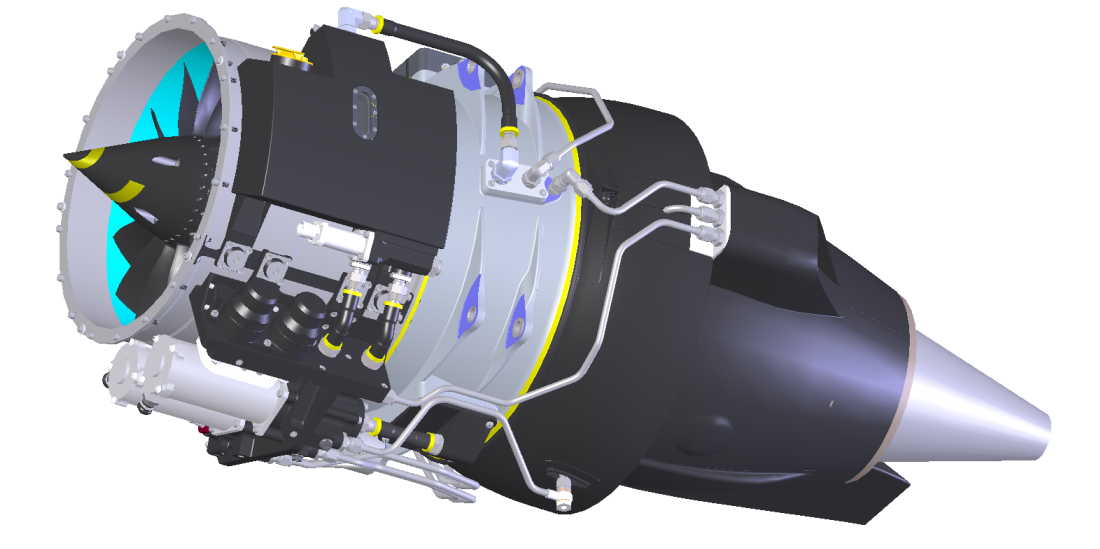
\includegraphics[scale=0.5,trim={0 0.2cm 0 0}]{fig/DGEN380.png}
  \caption{le Turboréacteur DGEN 380}
\end{figure}

\chapter{Réalisation du projet}

Tout d’abord, afin d’utiliser le moteur turbofan DGEN 380 nous avons besoin
d’une loi de commande qui va permettre de gérer le moteur afin d’atteindre
une certaine vitesse. Dans notre cas, nous essayons de nous rapprocher au
maximum du fonctionnement réel du moteur. Nous avons à notre disposition
sur SimuLink, le modèle réel utilisé pour simuler le comportement dynamique
du moteur. A partir de cela nous construisons 
autour de cette base une loi de commande qui permettra d’avoir les résultats
correspondants aux réactions réelles du système. Pour cela, il existe plusieurs
moyens de la trouver, ces solutions seront plus ou moins précises suivant la 
façon dont elles sont trouvées.

\begin{figure}[!h]
  \vspace{1cm}
  \centering
  \includegraphics[scale=0.37, trim={0.2cm 0 0 0}]{fig/système_simulink.png}
  \caption{Modèle "boîte noire" du turboréacteur DGEN 380 dans Simulink}
  \vspace{0.5cm}
\end{figure}

\newpage

\section{Analyse du système}
Dans cette partie, l’objectif est de déterminer une approximation linéaire du 
système de manière à pouvoir l’utiliser pour déterminer les lois de commande.  
Pour cela, la première étape consiste à s’assurer que le système est stable. 
Sinon nous ne pouvons pas faire d’approximation linéaire.
On trace donc la réponse temporelle pour un échelon d’amplitude 50.

\begin{figure}[!h]
  \vspace{1cm}
  \centering
  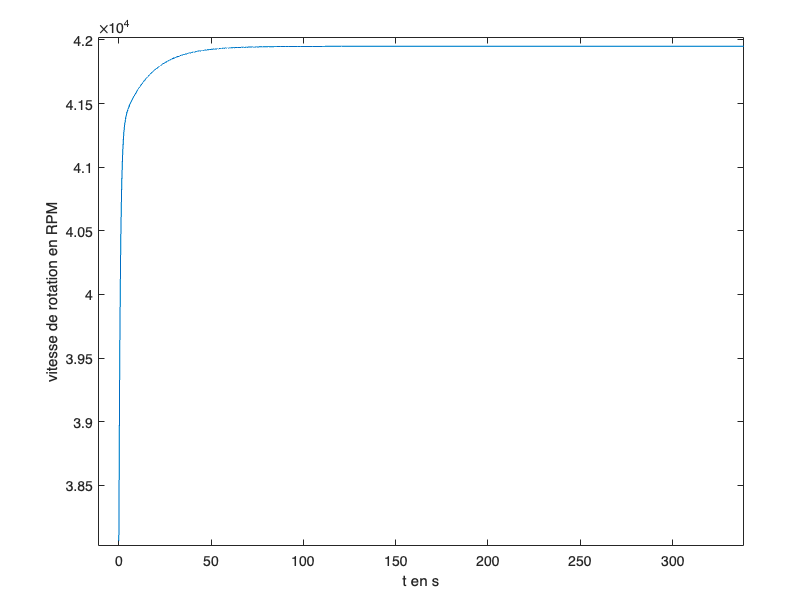
\includegraphics[scale=0.35]{fig/step_response.png}
  \caption{Réponse temporelle du système à un échelon d'amplitude 50}
  \vspace{0.5cm}
\end{figure}

On constate alors que la courbe tend vers une asymptote. Cela signifie que le
système est stable.
Ensuite on étudie l’effet sur le système de la variation des différents
paramètres : $h(t)$ l’altitude à laquelle se trouve l’avion en mètres, $v(t)$ la 
vitesse en Mach et $T(t)$ la différence de température. On trace donc la même 
réponse temporelle avec tous les paramètres constants et on fait plusieurs courbes 
avec différentes valeurs de $\Delta T$

\begin{figure}[!h]
  \vspace{1cm}
  \centering
  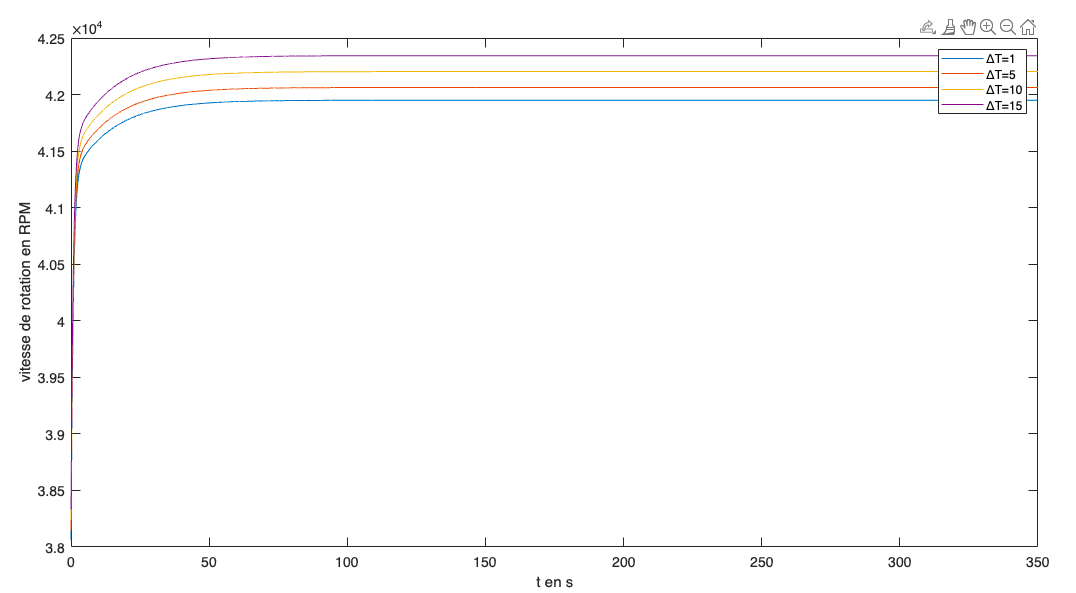
\includegraphics[scale=0.3]{fig/step_response_deltaT.png}
  \caption{Réponses temporelles du système pour des valeurs de $\Delta T$ différentes}
  \vspace{0.2cm}
\end{figure}

On choisit alors de fixer $T(t) = 1\Delta_{ISA}$ pour le reste de l'étude et on
trace les mêmes réponses pour des variations de $h(t)$ et $v(t)$.

\begin{figure}[!h]
  \vspace{1cm}
  \centering

  \begin{tabular}{cc}
    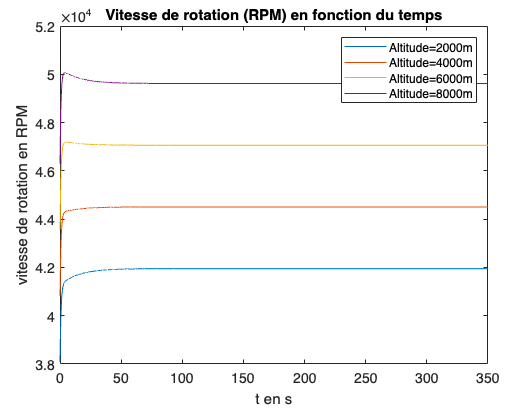
\includegraphics[width=0.45\linewidth]{fig/step_response_h.png} &
    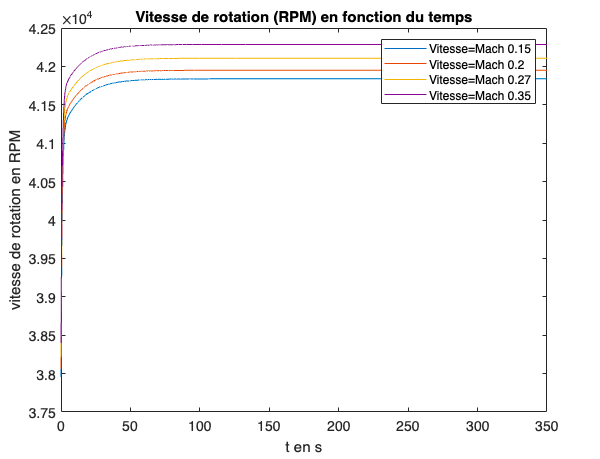
\includegraphics[width=0.45\linewidth]{fig/step_response_v.png} \\
  \end{tabular}
  \caption{Réponses temporelles du système pour des valeurs de $v(t)$ et $h(t)$ différentes}
  \vspace{0.5cm}
\end{figure}

On choisit de fixer $h(t) = 2000m$ et $v(t) = 0.2 ~ Mach$ pour le reste de l'étude.
Il faut ensuite trouver la valeur du point d'équilibre pour les constantes choisies.
On trace la réponse temporelle du système à un échelon de 50 pour $h(t) = 2000m$, 
$v(t) = 0.2 ~ Mach$ et $T(t) = 1\Delta_{ISA}$.

\begin{figure}[!h]
  \vspace{1cm}
  \centering
  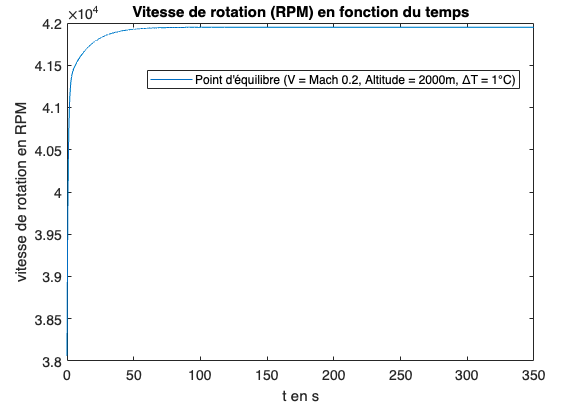
\includegraphics[scale=0.7]{fig/step_response_equilibre.png}
  \caption{Réponse temporelle du système à un échelon d'amplitude 50 pour les constantes choisies}
  \vspace{0.5cm}
\end{figure}

Le point d'équilibre du système pour les constantes choisies est donc de $y = 41950 ~ RPM$
L'étape suivante consiste à déterminer un échelon dont la réponse du système est 
proche de la réponse d'un système linéaire. Il faut alors tracer deux réponses indicielles
pour deux échelons d'amplitude $\Delta = 10$ et $\Delta = 20$.

Pour mieux visualiser la différence, on remet les axes à zéro et on met à l'échelle
un demi la réponse à l'échelon d'amplitude $\Delta = 20$.

\begin{figure}[!h]
  \vspace{0.3cm}
  \centering
  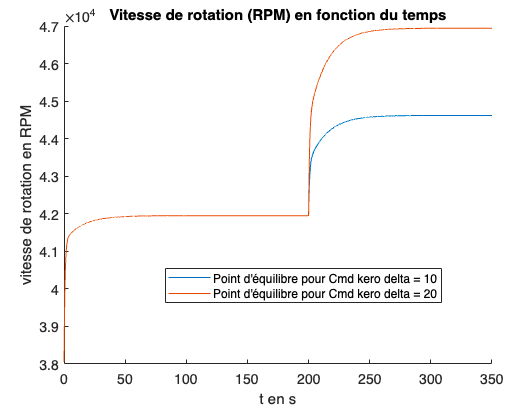
\includegraphics[scale=0.55]{fig/step_response_delta10-20.png}
  \caption{Réponses temporelles du système à des échelons d'amplitude 10 et 20}
  \vspace{0.7cm}
  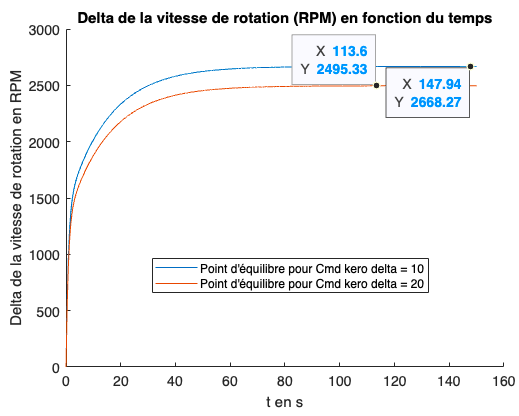
\includegraphics[scale=0.55]{fig/step_response_delta10-20_scaled.png}
  \caption{Réponses temporelles du système à des échelons d'amplitude 10 et 20 mises à l'échelle}
  \vspace{0.3cm}
\end{figure}

Dans un système linéaire, les deux courbes des réponses mises à l'échelles doivent 
être superposées. Or ce n'est pas le cas ici, on observe une différence de $172$ entre
les deux valeurs d'équilibre. On en déduit alors que le système qui modélise le DGEN 380
n'est pas linéaire. Il va alors falloir procéder à un approximation du système par un
système linéaire lors de la modélisation.


\newpage


\section{Modélisation du système}

\subsection{Modélisation par analyse temporelle}

Lors de la modélisation du turboréacteur, une valeur d'échelon de $\Delta = 1$ 
sera choisie car autour de cette valeur, le comportement du système est quasi-linéaire.
Ce qui permettra de simplifier la modélisation du système.

\begin{figure}[!h]
  \vspace{1cm}
  \centering
  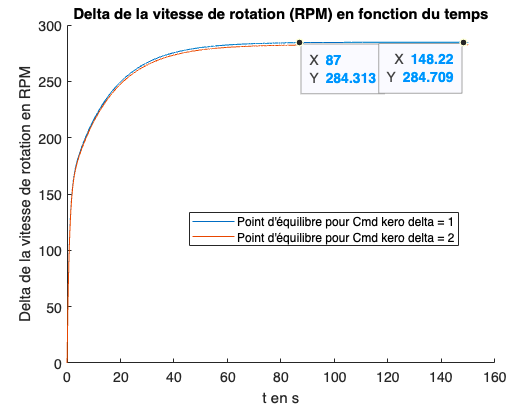
\includegraphics[scale=0.7]{fig/step_response_delta1-2_scaled.png}
  \caption{Réponses temporelles du système à des échelons d'amplitude 1 et 2 mises à l'échelle}
\end{figure}

On peut alors commençer à modéliser le système par une fonction de transfert 
du premier ordre de la forme:

\begin{equation}
  G(p) = \frac{K}{p + \tau}
\end{equation}
\vspace{0.5cm}

où $K$ est le gain statique du système et $\tau$ le temps de réponse du système.

D'après le tracé de la réponse indicielle, on peut déterminer la valeur de 
$K$ et de $\tau$.

On trouve pour un échelon de $\Delta = 1$: 

\begin{equation}
  \left\{
  \begin{matrix}
    K = 142.35 \\
    \tau = 1.77 ~ s
  \end{matrix}
  \right.
\end{equation}
\vspace{0.5cm}

On peut alors tracer la réponse indicielle de cette première approximation du système.

\newpage

\begin{figure}[!h]
  \vspace{0.5cm}
  \centering
  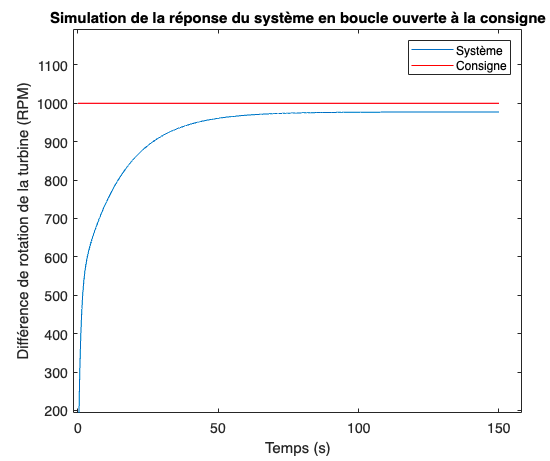
\includegraphics[scale=0.7]{fig/step_response_delta1_approximation.png}
  \caption{Réponse temporelle du système à un échelon d'amplitude 1 avec la première approximation}
\end{figure}

On constate que la première approximation du système est incorrecte. Il faut alors utiliser
une autre méthode pour déterminer un modèle plus précis.



\subsection{Modélisation par analyse fréquentielle}

Pour modéliser la fonction de transfert du système avec plus de précision, on va
effectuer une analyse fréquentielle du système. On va donc récupérer les valeurs de 
gain et de déphasage du système pour différentes fréquences en entrée.

\begin{equation}
\footnotesize
\begin{tabular}{| l | c | c | c | c | c | c | c | c | c | r |}
  \hline
  Pulsation $rad/s^{-1}$ & $10^{-3}$ & $10^{-2}$ & $4 \cdot 10^{-2}$ & $10^{-1}$ & $2 \cdot 10^{-1}$ & $5 \cdot 10^{-1}$ & $ 10 $ & $ 3 \cdot 10 $ & $ 10^1 $ & $ 3 \cdot 10^1 $  \\
  \hline
  Gain & 268.5 & 284.2 & 276 & 206 & 174.2 & 150 & 124.6 & 60 & 17 & 3.66 \\
  Gain $dB$ & 48.5 & 49 & 48 & 46 & 44 & 43 & 41.9 & 35.5 & 24 & 11.26 \\
  Décalage $s$ & 3.9 & 6.2 & 5.9 & 3.7 & 2.12 & 1 & 0.752 & 0.437 & 0.713 & 0.06 \\
  Phase (degrés) & -0.22 & -3.5 & -13.5 & -21.2 & -24.29 & -28.6 & -43 & -75 & -99 & -103 \\
  \hline
\end{tabular}
\end{equation}

Après avoir obtenu les valeurs de ce tableau, on peut tracer un diagramme de Bode pour
déterminer l'ordre du système et les valeurs des constantes de ce dernier. On fait 
coincider la courbe de la réponse fréquentielle du système avec celle de notre approximation
afin de déterminer les constantes du système.

\newpage

\begin{figure}[!h]
  \centering
  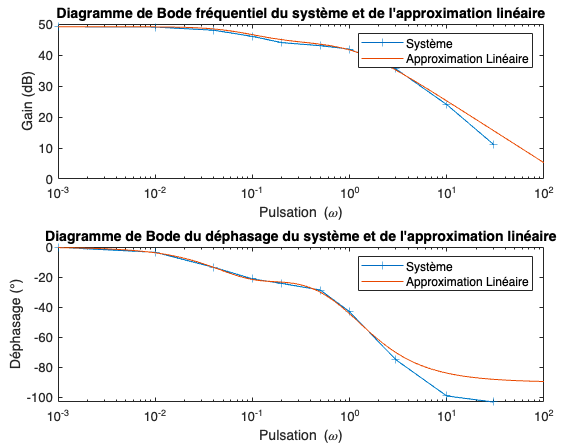
\includegraphics[scale=0.7]{fig/bode_diagram.png}
  \caption{Diagramme de Bode du système et de l'approximation d'ordre 3}
  \vspace{0.5cm}
\end{figure}

On trouve alors que le système est d'ordre 3, de forme:

\vspace{0.5cm}
\begin{equation}
  G(p) = \frac{K}{(p + \tau_1)(p + \tau_2)(p + \tau_3)}
\end{equation}
\vspace{0.5cm}

et possède donc 3 constantes de temps nommées
$\tau_1$, $\tau_2$ et $\tau_3$ où :

\vspace{0.5cm}
\begin{equation}
  \left\{
  \begin{matrix}
    \tau_1 = 0.0135 \\
    \tau_2 = 0.075 \\
    \tau_3 = 1.1 \\
    K = 268.5
  \end{matrix}
  \right.
\end{equation}
\vspace{0.5cm}

\newpage

\section{Systèmes de commande en boucle ouverte}

Après cette modélisation du comportement du turboréacteur. On obtient une 
fonction de transfert utilisable de la forme:

\begin{equation}
  G(p) = \frac{\Delta Y(p)}{\Delta U(p)}
\end{equation}

Grâce à cette fonction de transfert, on peut alors déterminer une loi de commade afin
d'amener la vitesse à une valeur de référence $\Delta y(t)$ aussi appelée consigne $\Delta r(t)$.
Cette consigne représente la vitesse souhaitée par l'utilisateur autour du point d'équilibre.

\begin{figure}[h]
  \centering
  \vspace{0.2cm}
  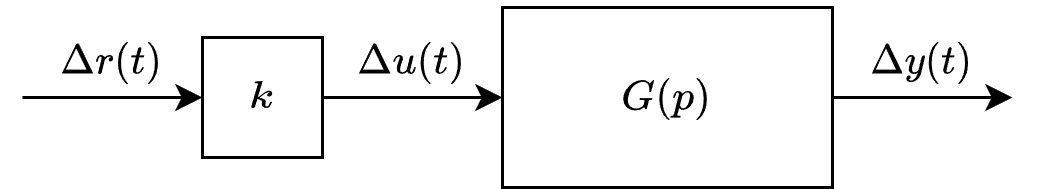
\includegraphics[scale=0.25]{fig/open_loop_system.png}
  \caption{Schéma d'un système en boucle ouverte}
\end{figure}

On sait qu'en régime permanent la consigne est égale à la sortie du système, et que
la sortie du système est égale à la valeur de référence multipliée par le gain
statique du système. Soit :

\begin{equation}
  \left\{
  \begin{matrix}
    \Delta u(t) = K \cdot \Delta y(t) \\
    \Delta y(t) = \Delta r(t)
  \end{matrix}
  \right.
\end{equation}

On peut alors déterminer aisément la valeur de $k$. On obtient alors: $k = \frac{1}{K} = 3.49 \cdot 10^{-3}$

Avec ces valeurs on peut alors tester la loi de commande en boucle ouverte 
pour une consigne de $\Delta r(t) = 1000 ~ RPM$, ce qui revient à amener la vitesse
de rotation du moteur à 1000 tours par minute au dessus de sa vitesse d'équilibre.

\begin{figure}[!h]
  \centering
  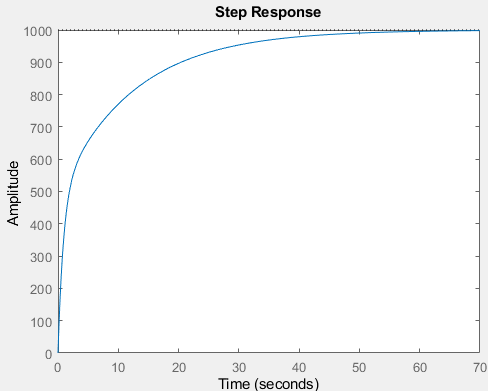
\includegraphics[scale=0.7]{fig/open_loop_response.png}
  \caption{Réponse du système à la loi de commande en boucle ouverte}
\end{figure}

À partir de ce système on peut déterminer le temps de réponse du système, 
c'est à dire le temps nécessaire au système pour atteindre 95\% de sa valeur finale
après un changement de consigne. On obtient alors un temps de réponse $T_{95\%} = 29.1s$.
Cependant, en substituant le modèle par le turboréacteur on constate que la 
valeur finale n'est pas de 1000 tours par minute mais de 974 tours par minute.
Cette légère différence est due au fait que le modèle est une approximation
du système et donc ne prend pas en compte les effets non linéaires du système.

\section{Système de commande en boucle fermée}

\subsection{Loi de commande proportionelle}

Pour améliorer le comportement du système, on peut ajouter une rétro-action dans la
loi de commande, transformant ainsi le système en une boucle fermée. Cette rétro-action
permet de corriger les erreurs de mesure du système et donc d'améliorer sa réponse.

\begin{figure}[h]
  \centering
  \vspace{0.3cm}
  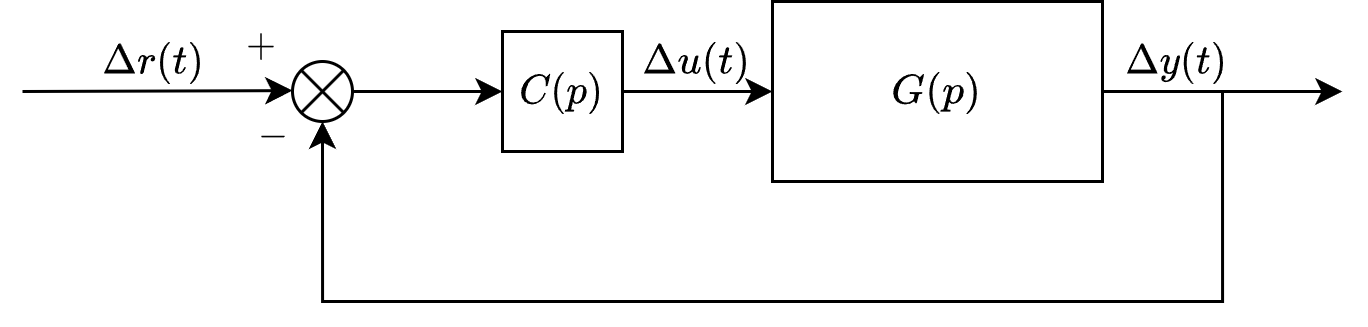
\includegraphics[scale=0.25]{fig/closed_loop_system.png}
  \caption{Schéma d'un système en boucle fermée}
\end{figure}

\begin{figure}[h]
  \centering
  \vspace{0.3cm}
  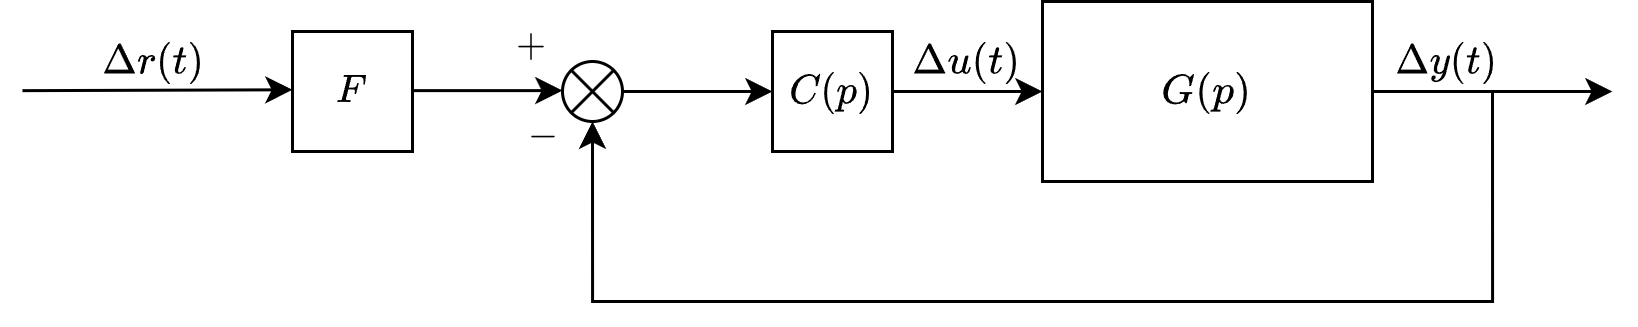
\includegraphics[scale=0.25]{fig/closed_loop_system_w-precomp.png}
  \caption{Schéma d'un système en boucle fermée avec précompensateur}
\end{figure}

Un correcteur proportionel est utilisé premièrement dans la boucle rétro-active
afin de corriger les erreurs de mesure. On obtient alors la loi de commande suivante:

\vspace{0.1cm}
\begin{equation}
  \Delta u(t) = k_p \cdot \Delta e(t)
\end{equation}
\vspace{0.1cm}

La transformée de Laplace de ce correcteur proportionel étant :

\vspace{0.1cm}
\begin{equation}
  C(p) = K_p
\end{equation}
\vspace{0.1cm}

Grâce à l'outil $Sisotools$ de $MATLAB$ on peut alors déterminer le gain
proportionnel $k_p$ de la loi de commande. On obtient alors $k_p = 0.0096$.
En utilisant cette valeur on peut alors tester la loi de commande en boucle fermée
pour une consigne de $\Delta r(t) = 1000 ~ RPM$. On obtient alors une valeur en régime
permanent de $\Delta y_{\infty} = 732 ~ RPM$, et un temps de réponse $T_{95\%} = 10s$.
Malgré une amélioration du temps de réponse, il reste toujours une différence entre
la consigne et la valeur finale. Pour remédier à cela, on ajoute un précompensateur
à la consigne afin de réduire cette différence. On obtient alors la loi de commande

\vspace{0.2cm}
\begin{equation}
  \Delta u(t) = k_p \cdot (F \cdot \Delta r(t) - \Delta y(t))
\end{equation}
\vspace{0.2cm}

En réglant la valeur du précompensateur $F$ on peut alors obtenir une valeur en régime
permanent de $\Delta y_{\infty} = 1000 ~ RPM$ pour une valeur de $F = 1.35$. Le gain
statique de la loi de commande est alors bien égale à 1.

\newpage

\subsection{Loi de commande intégrale}

Dans un second temps on retire le précompensateur et on remplace le correcteur proportionnel par un correcteur intégral.
On obtient alors la loi de commande suivante: 

\vspace{0.2cm}
\begin{equation}
  \Delta u(t) = k_i \cdot \int_{0}^{t} \Delta e(t) dt
\end{equation}

La transformée de Laplace de cet intégrateur étant :

\vspace{0.2cm}
\begin{equation}
  C(p) = \frac{1}{T_i \cdot p}
\end{equation}


L'utilisation d'un intégrateur permet de réduire le temps de réponse du système
en réduisant l'erreur de mesure. Grâce à $Sisotools$ on obtient alors un gain intégral
$k_i = 0.00089303$. En utilisant cette valeur on peut alors tester la loi de commande
en boucle fermée pour une consigne de $\Delta r(t) = 1000 ~ RPM$. Le temps de réponse
est légèrement amélioré et l'erreur de mesure est éliminée.

\subsection{Loi de commande proportionelle intégrale}

Enfin, en combinant les correcteurs proportionnel et intégral, on obtient la loi de 
commande suivante:

\vspace{0.2cm}
\begin{equation}
  \Delta u(t) = k_p \cdot \Delta e(t) + k_i \cdot \int_{0}^{t} \Delta e(t) dt
\end{equation}

La transformée de Laplace de cette loi de commande étant :

\vspace{0.2cm}
\begin{equation}
  C(p) = K_p \cdot \left( 1 + \frac{1}{T_i \cdot p} \right)
\end{equation}

Grâce à $Sisotools$ on peut alors déterminer les valeurs de $K_p$ et $T_i$ afin d'avoir
une loi de commande plus précise avec un temps de réponse moindre. On obtient alors :

\vspace{0.2cm}
\begin{equation}
  \left\{
  \begin{matrix}
  K_p = 0.009213 \\
  T_i = 1.1765
  \end{matrix}
  \right.
\end{equation}

Ces valeurs permettent alors d'obtenir un temps de réponse de $T_{95\%} = 2.5s$ dans
le cas d'utilisation de la boite noire. Cette loi de commande permet dont d'obtenir 
une réponse très rapide du système et une erreur de mesure nulle.

\newpage

\chapter{Conclusion}

L'objectif principal de ce projet était de mettre en place une loi de commande
d'un petit turboréacteur, le DGEN 380. Cette loi de commande devait permettre de
contrôler la vitesse de rotation de la turbine et de lier l'entrée en carburant
pour obtenir la valeur désirée. Au cours de ce projet, nous avons pu nous familiariser
avec les différents outils logiciels utilisés dans ce domaine, notamment $MATLAB$,
$Simulink$ et $Sisotools$. Nous avons appris à l'aide de ces logiciels à mettre 
en place la modélisation d'un système, à simuler ce système et à créer un loi de
commande et un correcteur proportionel et/ou intégral. Nous avons pu ainsi mettre
en application la théorie vue en cours et en TD de $DSL$.




\end{document}